\documentclass{beamer}
\usepackage[utf8]{inputenc}

\usetheme{Madrid}
\usecolortheme{default}
\usepackage{amsmath,amssymb,amsfonts,amsthm}
\usepackage{mathtools}
\usepackage{txfonts}
\usepackage{tkz-euclide}
\usepackage{listings}
\usepackage{adjustbox}
\usepackage{array}
\usepackage{gensymb}
\usepackage{tabularx}
\usepackage{gvv}
\usepackage{lmodern}
\usepackage{circuitikz}
\usepackage{tikz}
\lstset{literate={·}{{$\cdot$}}1 {λ}{{$\lambda$}}1 {→}{{$\to$}}1}
\usepackage{graphicx}

\setbeamertemplate{page number in head/foot}[totalframenumber]

\usepackage{tcolorbox}
\tcbuselibrary{minted,breakable,xparse,skins}



\definecolor{bg}{gray}{0.95}
\DeclareTCBListing{mintedbox}{O{}m!O{}}{%
  breakable=true,
  listing engine=minted,
  listing only,
  minted language=#2,
  minted style=default,
  minted options={%
    linenos,
    gobble=0,
    breaklines=true,
    breakafter=,,
    fontsize=\small,
    numbersep=8pt,
    #1},
  boxsep=0pt,
  left skip=0pt,
  right skip=0pt,
  left=25pt,
  right=0pt,
  top=3pt,
  bottom=3pt,
  arc=5pt,
  leftrule=0pt,
  rightrule=0pt,
  bottomrule=2pt,
  toprule=2pt,
  colback=bg,
  colframe=orange!70,
  enhanced,
  overlay={%
    \begin{tcbclipinterior}
    \fill[orange!20!white] (frame.south west) rectangle ([xshift=20pt]frame.north west);
    \end{tcbclipinterior}},
  #3,
}
\lstset{
    language=C,
    basicstyle=\ttfamily\small,
    keywordstyle=\color{blue},
    stringstyle=\color{orange},
    commentstyle=\color{green!60!black},
    numbers=left,
    numberstyle=\tiny\color{gray},
    breaklines=true,
    showstringspaces=false,
}
%------------------------------------------------------------
%This block of code defines the information to appear in the
%Title page
\title %optional
{10.4.2}
\date{September 11,2025}
%\subtitle{A short story}

\author % (optional)
{Harsha-EE25BTECH11026}



\begin{document}


\frame{\titlepage}


\begin{frame}{Question}
Find the equations of tangent and normal to the curve $y=\frac{x-7}{\brak{x-2}\brak{x-3}}$ at the point where it cuts the X axis.
\end{frame}

\begin{frame}{Theoretical Solution}
It is given that the tangents and normal are drawn at the point where the curve intersects the X axis i.e, at $\vec{P}=\myvec{7\\0}$ 
Let the equations of tangent be,
\begin{align}
    \vec{n_1}^{\top}\vec{x}=c_1 \label{eq:1}
\end{align}
And equation of normal be,
\begin{align}
    \vec{n_2}^{\top}\vec{x}=c_2 \label{eq:2}
\end{align}
To solve for their direction vectors, we can use he Jacobian technique.

\end{frame}

\begin{frame}{Theoretical Solution}
It states that,
\begin{align}
    \vec{n}=\myvec{\frac{\partial{F}}{\partial{x}}\\\frac{\partial{F}}{\partial{y}}}_{\text{at point of tangency}}
\end{align}
where,
\begin{align*}
    \vec{n}:\text{Direction vector of tangent}\\
    \vec{F(x,y)}:\text{Function of the curve}
\end{align*}
Equation of the curve can be modified and written as,
\begin{align}
    yx^2-5xy+6y-x+7=0
\end{align}
\begin{align}
    \implies \vec{n}=\myvec{2xy-5y-1\\x^2-5x+6}
\end{align}

\end{frame}

\begin{frame}{Theoretical Solution}
Substituting the point $\vec{P}$,
\begin{align}
    \therefore \vec{n_1}=\myvec{-1\\20} \label{eq:3}
\end{align}
\begin{align}
    \implies \vec{n_2}=\myvec{20\\1} \label{eq:4}
\end{align}
Substituing ~\eqref{eq:3} and ~\eqref{eq:4} in ~\eqref{eq:1} and ~\eqref{eq:2} respectively yields,
\begin{align}
    \myvec{-1&&20}\vec{x}=c_1 \label{eq:5} \\
    \myvec{20&&1}\vec{x}=c_2 \label{eq:6}
\end{align}
Substituting $\vec{P}$ in ~\eqref{eq:5} and ~\eqref{eq:6},
\begin{align}
    \implies c_1=-7 \quad and \quad c_2=140
\end{align}

\end{frame}

\begin{frame}{Theoretical Solution}
\begin{align}
    \therefore \text{Equation of tangent:} \myvec{-1&&20}\vec{x}=-7
\end{align}
\begin{align}
    \therefore \text{Equation of normal:} \myvec{20&&1}\vec{x}=140
\end{align}

\end{frame}

\begin{frame}[fragile]
    \frametitle{C Code -Finding the intersection of conics}

    \begin{lstlisting}[language=C]
#include <stdio.h>
#include <math.h>

// Function to evaluate the curve y = (x-7)/((x-2)(x-3))
double curve(double x) {
    double denom = (x - 2.0) * (x - 3.0);
    if (fabs(denom) < 1e-9) {
        return NAN; // return NaN at asymptotes
    }
    return (x - 7.0) / denom;
}

// Function to evaluate tangent line at (7,0)
double tangent(double x) {
    double m_tan = 1.0 / 20.0; // slope of tangent
    return m_tan * (x - 7.0);
}
    \end{lstlisting}
\end{frame}

\begin{frame}[fragile]
    \frametitle{C Code -Finding the intersection of conics}

    \begin{lstlisting}[language=C]
// Function to evaluate normal line at (7,0)
double normal(double x) {
    double m_norm = -20.0; // slope of normal
    return m_norm * (x - 7.0);
}

// Function to print tangent & normal equations
void print_equations() {
    double m_tan = 1.0 / 20.0;
    double m_norm = -20.0;

    printf("Tangent equation: y = %.1f*(x - 7)\n", m_tan);
    printf("Normal equation:  y = %.1f*(x - 7)\n", m_norm);
}
\end{lstlisting}
\end{frame}




\begin{frame}[fragile]
    \frametitle{Python+C code}

    \begin{lstlisting}[language=Python]
import ctypes
import numpy as np
import matplotlib.pyplot as plt

# Load C library
lib = ctypes.CDLL("./libcurve_solver.so")

# Function signatures
lib.curve.restype = ctypes.c_double
lib.curve.argtypes = [ctypes.c_double]
lib.tangent.restype = ctypes.c_double
lib.tangent.argtypes = [ctypes.c_double]
lib.normal.restype = ctypes.c_double
lib.normal.argtypes = [ctypes.c_double]
lib.print_equations.restype = None
    \end{lstlisting}
\end{frame}

\begin{frame}[fragile]
    \frametitle{Python+C code}

    \begin{lstlisting}[language=Python]
# Print equations once
lib.print_equations()

# Define helper wrappers for numpy arrays
def curve(x):
    return np.array([lib.curve(float(val)) for val in x])

def tangent(x):
    return np.array([lib.tangent(float(val)) for val in x])

def normal(x):
    return np.array([lib.normal(float(val)) for val in x])

# Split domain around asymptotes
x_vals1 = np.linspace(-2, 1.9, 200)
x_vals2 = np.linspace(2.1, 2.9, 200)
x_vals3 = np.linspace(3.1, 12, 200)

    \end{lstlisting}
\end{frame}

\begin{frame}[fragile]
    \frametitle{Python+C code}

    \begin{lstlisting}[language=Python]
y_vals1 = curve(x_vals1)
y_vals2 = curve(x_vals2)
y_vals3 = curve(x_vals3)

# Tangent & normal
x0, y0 = 7, 0
x_line = np.linspace(4, 10, 200)
y_tan = tangent(x_line)
y_norm = normal(x_line)

plt.figure(figsize=(8,6))
plt.plot(x_vals1, y_vals1, 'b')
plt.plot(x_vals2, y_vals2, 'b')
    \end{lstlisting}
\end{frame}

\begin{frame}[fragile]
    \frametitle{Python+C code}

    \begin{lstlisting}[language=Python]
plt.plot(x_vals3, y_vals3, 'b', label="Curve y=(x-7)/((x-2)(x-3))")
plt.plot(x_line, y_tan, 'r--', label="Tangent at (7,0)")
plt.plot(x_line, y_norm, 'g--', label="Normal at (7,0)")
plt.scatter([x0], [y0], color='k', zorder=5)
plt.text(x0+0.2, y0+0.2, "(7,0)")
plt.axhline(0, color='gray', lw=1)
plt.axvline(0, color='gray', lw=1)
plt.ylim(-2, 2)
plt.xlim(-2, 12)
plt.xlabel("x")
plt.ylabel("y")
plt.legend()
plt.title("Curve with Tangent and Normal at (7,0)")
plt.grid(True)
plt.savefig("/home/user/Matrix Theory: workspace/Matgeo_assignments/10.4.2/figs/figure_1.png")
plt.show()

    \end{lstlisting}
\end{frame}

\begin{frame}[fragile]
    \frametitle{Python code}
    \begin{lstlisting}[language=Python]
import numpy as np
import matplotlib.pyplot as plt
# Define the curve y = (x-7)/((x-2)(x-3))
def curve(x):
    denom = (x - 2) * (x - 3)
    mask = np.isclose(denom, 0)   # True where denominator ~ 0
    y = (x - 7) / denom
    y[mask] = np.nan
    return y

x0, y0 = 7, 0
def grad_F(x, y):
    Fx = 2 * x * y - 5 * y - 1
    Fy = x**2 - 5*x + 6
    return np.array([Fx, Fy])

# Evaluate gradient at (7,0)
Fx, Fy = grad_F(x0, y0)
    \end{lstlisting}   
\end{frame}

\begin{frame}[fragile]
    \frametitle{Python code}
    \begin{lstlisting}[language=Python]
def tangent(x):
    return y0 + m_tan * (x - x0)

# Normal line: slope = -1/m_tan (perpendicular)
m_norm = -1 / m_tan
def normal(x):
    return y0 + m_norm * (x - x0)

# Print equations
def print_equations():
    print(f"Tangent equation: y = {m_tan:.1f}*(x - {x0}) + {y0}")
    print(f"Normal equation:  y = {m_norm:.1f}*(x - {x0}) + {y0}")

print_equations()

    \end{lstlisting}   
\end{frame}

\begin{frame}[fragile]
    \frametitle{Python code}
    \begin{lstlisting}[language=Python]
# Plot
x_vals1 = np.linspace(-2, 1.9, 200)
x_vals2 = np.linspace(2.1, 2.9, 200)
x_vals3 = np.linspace(3.1, 12, 200)
y_vals1 = curve(x_vals1)
y_vals2 = curve(x_vals2)
y_vals3 = curve(x_vals3)

plt.figure(figsize=(8,6))
# Curve
plt.plot(x_vals1, y_vals1, 'b')
plt.plot(x_vals2, y_vals2, 'b')
plt.plot(x_vals3, y_vals3, 'b')
# Tangent and normal (extended around x0)
x_line = np.linspace(4, 10, 200)
plt.plot(x_line, tangent(x_line), 'r--', label="Tangent at (7,0)")
plt.plot(x_line, normal(x_line), 'g--', label="Normal at (7,0)")
    \end{lstlisting}   
\end{frame}

\begin{frame}[fragile]
    \frametitle{Python code}
    \begin{lstlisting}[language=Python]
# Mark the point of tangency
plt.scatter([x0], [y0], color='k', zorder=5)
plt.text(x0+0.2, y0+0.2, "(7,0)")

# Axes and formatting
plt.axhline(0, color='gray', lw=1)
plt.axvline(0, color='gray', lw=1)
plt.ylim(-2, 2)
plt.xlim(-2, 12)
plt.xlabel("x")
plt.ylabel("y")
plt.legend()
plt.title("Curve with Tangent and Normal at (7,0)")
plt.grid(True)
plt.savefig("/home/user/Matrix Theory: workspace/Matgeo_assignments/10.4.2/figs/Figure_1.png")
plt.show()
    \end{lstlisting}   
\end{frame}

\begin{frame}{Plot}
    \begin{figure}[H]
    \centering
    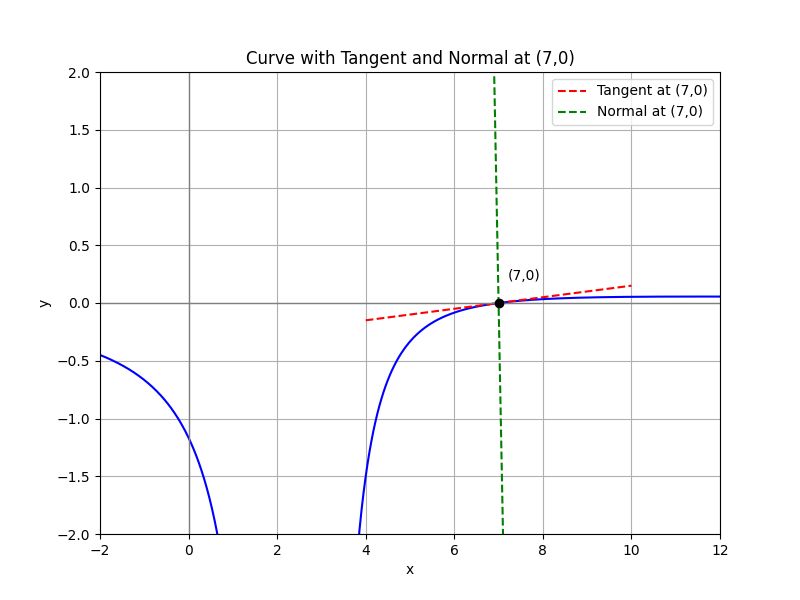
\includegraphics[width=0.6\columnwidth]{figs/Figure_1.png}
    \label{fig:1}
\end{figure}
\end{frame}

\end{document}